\documentclass[xcolor=dvipsnames]{beamer}
\usepackage[T1]{fontenc}
\usepackage[utf8]{inputenc}
\usepackage[english,slovak]{babel}

\usepackage{amsmath}
\usepackage{amsthm}
\usetheme{Pittsburgh}
\useoutertheme{shadow}

\usepackage{graphicx}
\usepackage{caption}
\usepackage{subcaption}

\usepackage[]{algorithm2e}
\usepackage{listings}
 \setbeamercovered{transparent}
 \usepackage{cuted}
\usepackage[export]{adjustbox}
\usepackage{mathtools}

\usepackage{lipsum}

\newcommand\Wider[2][3em]{%
\makebox[\linewidth][c]{%
  \begin{minipage}{\dimexpr\textwidth+#1\relax}
  \raggedright#2
  \end{minipage}%
  }%
}

%-------------------------------------------------------------------------------------
\title{\bf Stručne o súťažnej robotike}
\author{Michal CHOVANEC, PhD.}


%\setbeamertemplate{footline}[frame number]{}
\setbeamertemplate{navigation symbols}{}


\date[EURP]{\it Marec 2018}
\begin{document}

\begin{frame}
\titlepage
\centering{Fakulta riadenia a informatiky}
\end{frame}


\begin{frame}{\bf Stručne o súťažnej robotike}

\centering
\begin{figure}[htbp]
  \centering
    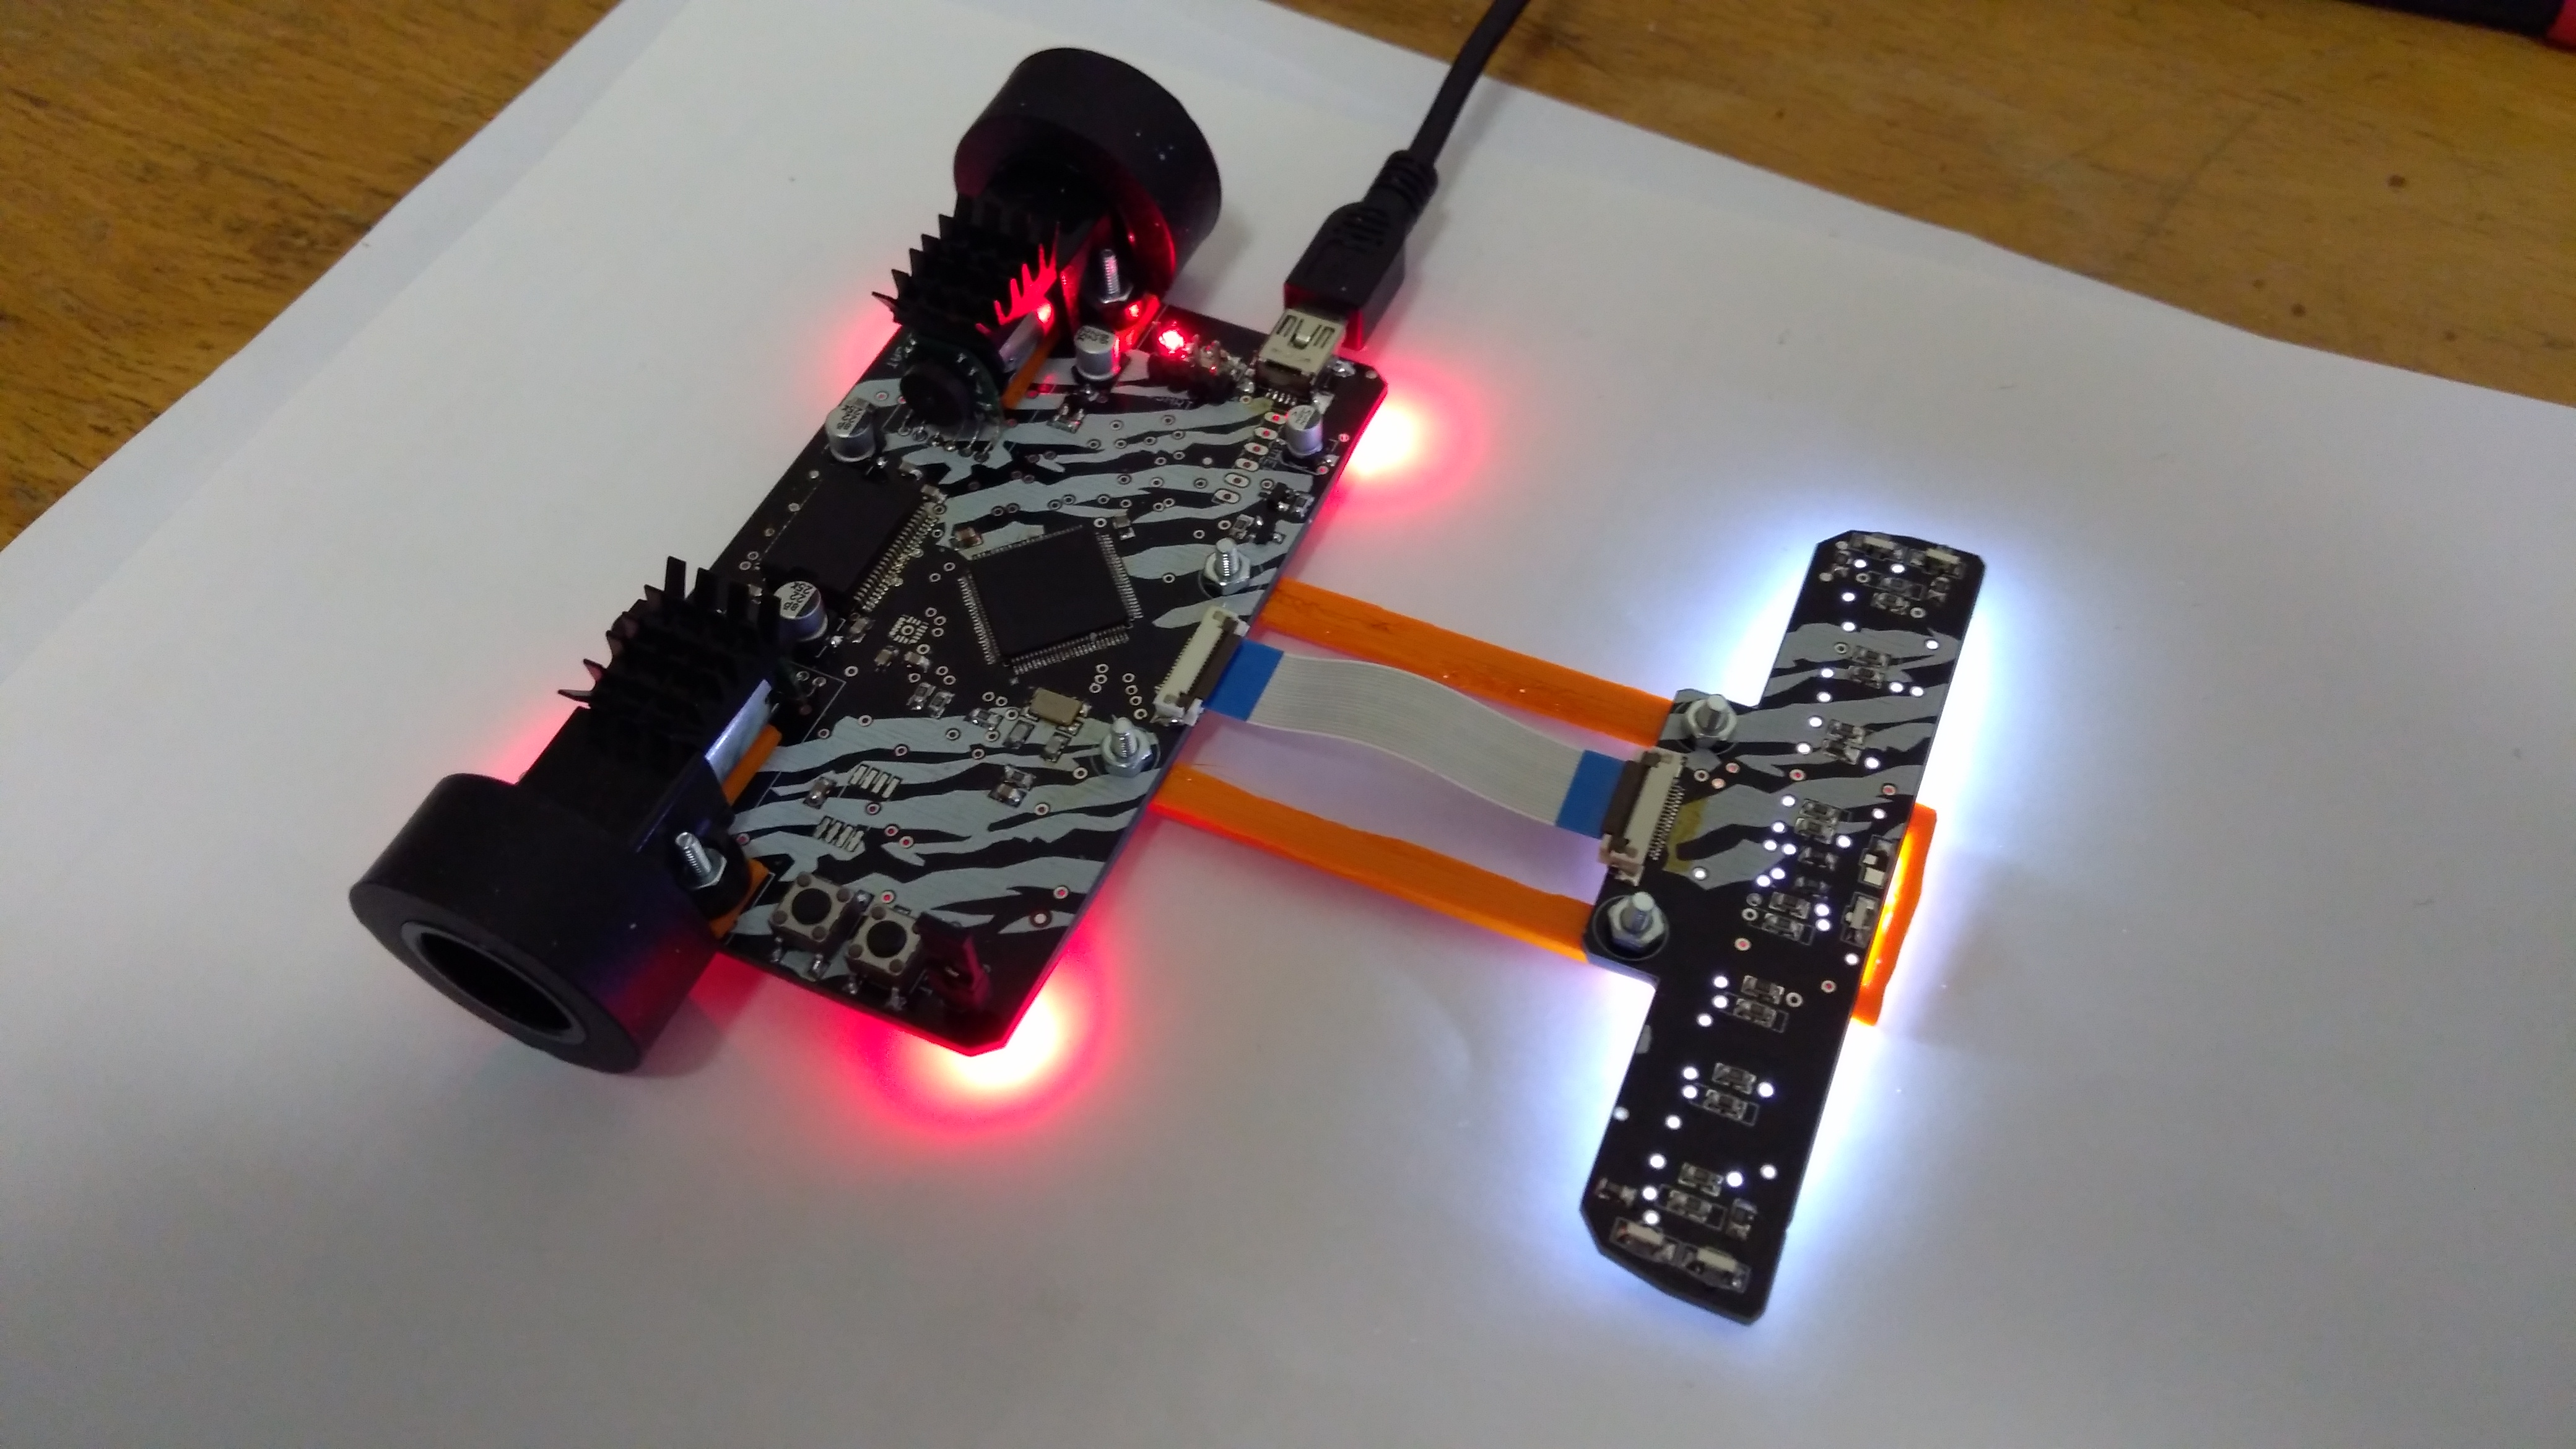
\includegraphics[scale=0.07]{ascender.jpg}
\end{figure}

\end{frame}



\begin{frame}{\bf Hardvér}
\Wider[4em]
{

\begin{minipage}[r]{0.5\textwidth}

\centering
\begin{figure}[htbp]
  \centering
    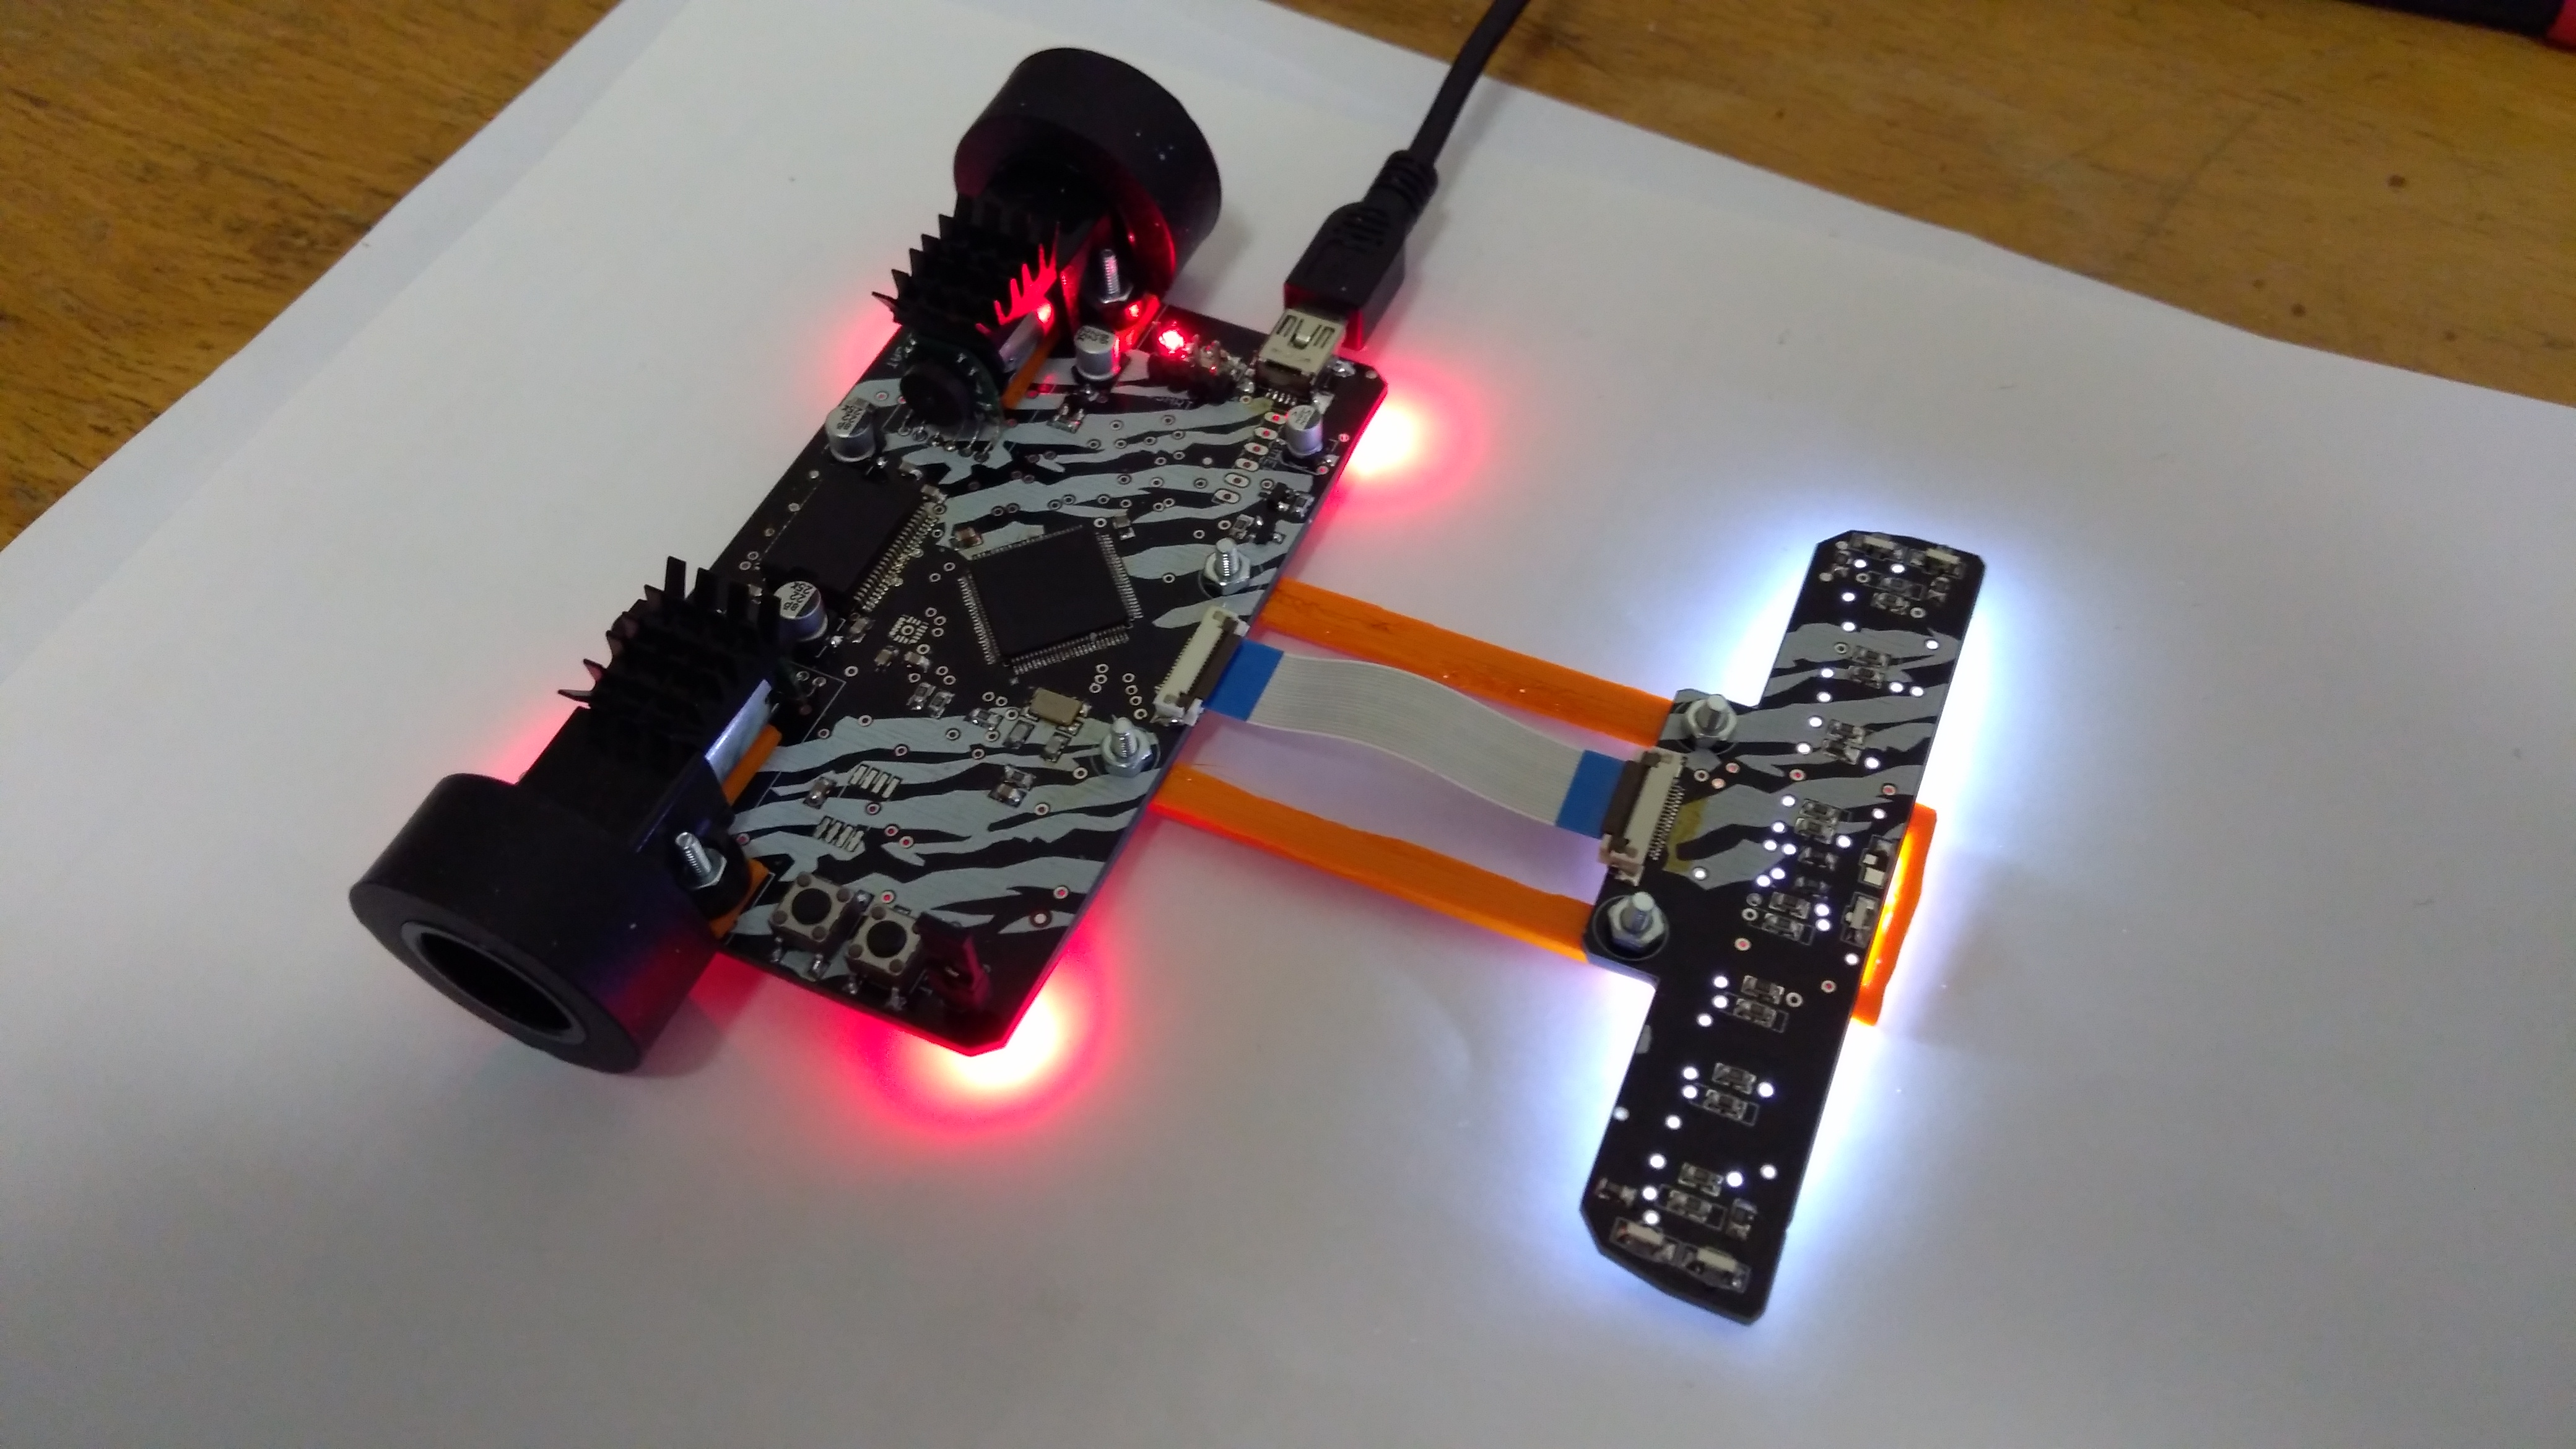
\includegraphics[scale=0.04]{ascender.jpg}
\end{figure}

\end{minipage}%
\hfill
\begin{minipage}[c]{0.5\textwidth}

\begin{itemize}
 \item procesor : ARM Cortex M7, 216MHz
 \item senzory  : 8x 500nm, 3xIR, gyroskop
 \item motory   : pololu, 1:30, micro metal HP
\end{itemize}

\end{minipage}%

}
\end{frame}



\begin{frame}{\bf Softvér}
\Wider[4em]
{

\begin{minipage}[r]{0.5\textwidth}

\centering
\begin{figure}[htbp]
  \centering
    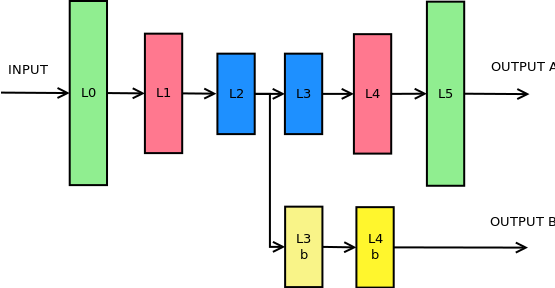
\includegraphics[scale=0.3]{nn.png}
\end{figure}

\centering
\begin{figure}[htbp]
  \centering
    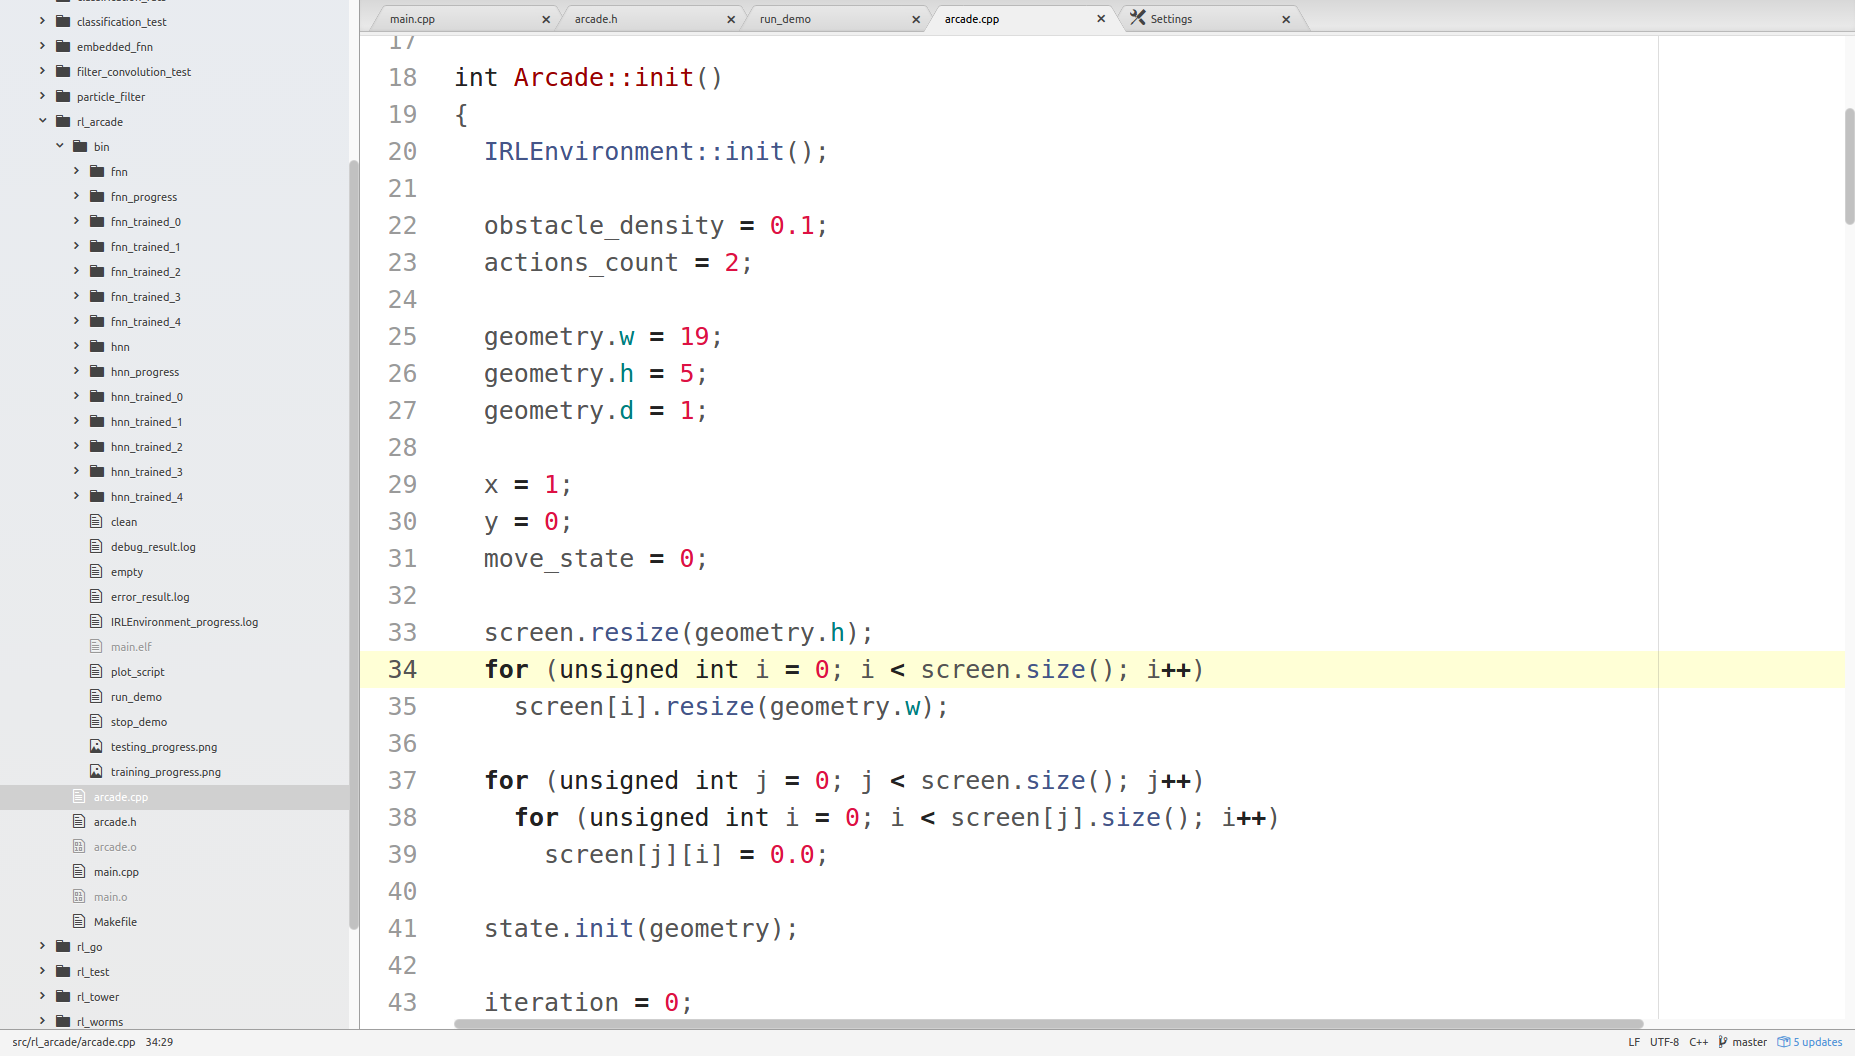
\includegraphics[scale=0.1]{code.png}
\end{figure}

\end{minipage}%
\hfill
\begin{minipage}[c]{0.5\textwidth}

\begin{itemize}
 \item ovládače : motory, senzory
 \item operačný systém : hard real time, max 5ms odozva
 \item inteligencia  : PID, PLL, neurónové siete, reinforcement learning
\end{itemize}

\end{minipage}%

}
\end{frame}




%-------------------------------------------------------------------------------------
\begin{frame}{\bf Q\&A}

\begin{figure}[ht]
\begin{center}
\begin{minipage}{0.8\linewidth}
\begin{center}
 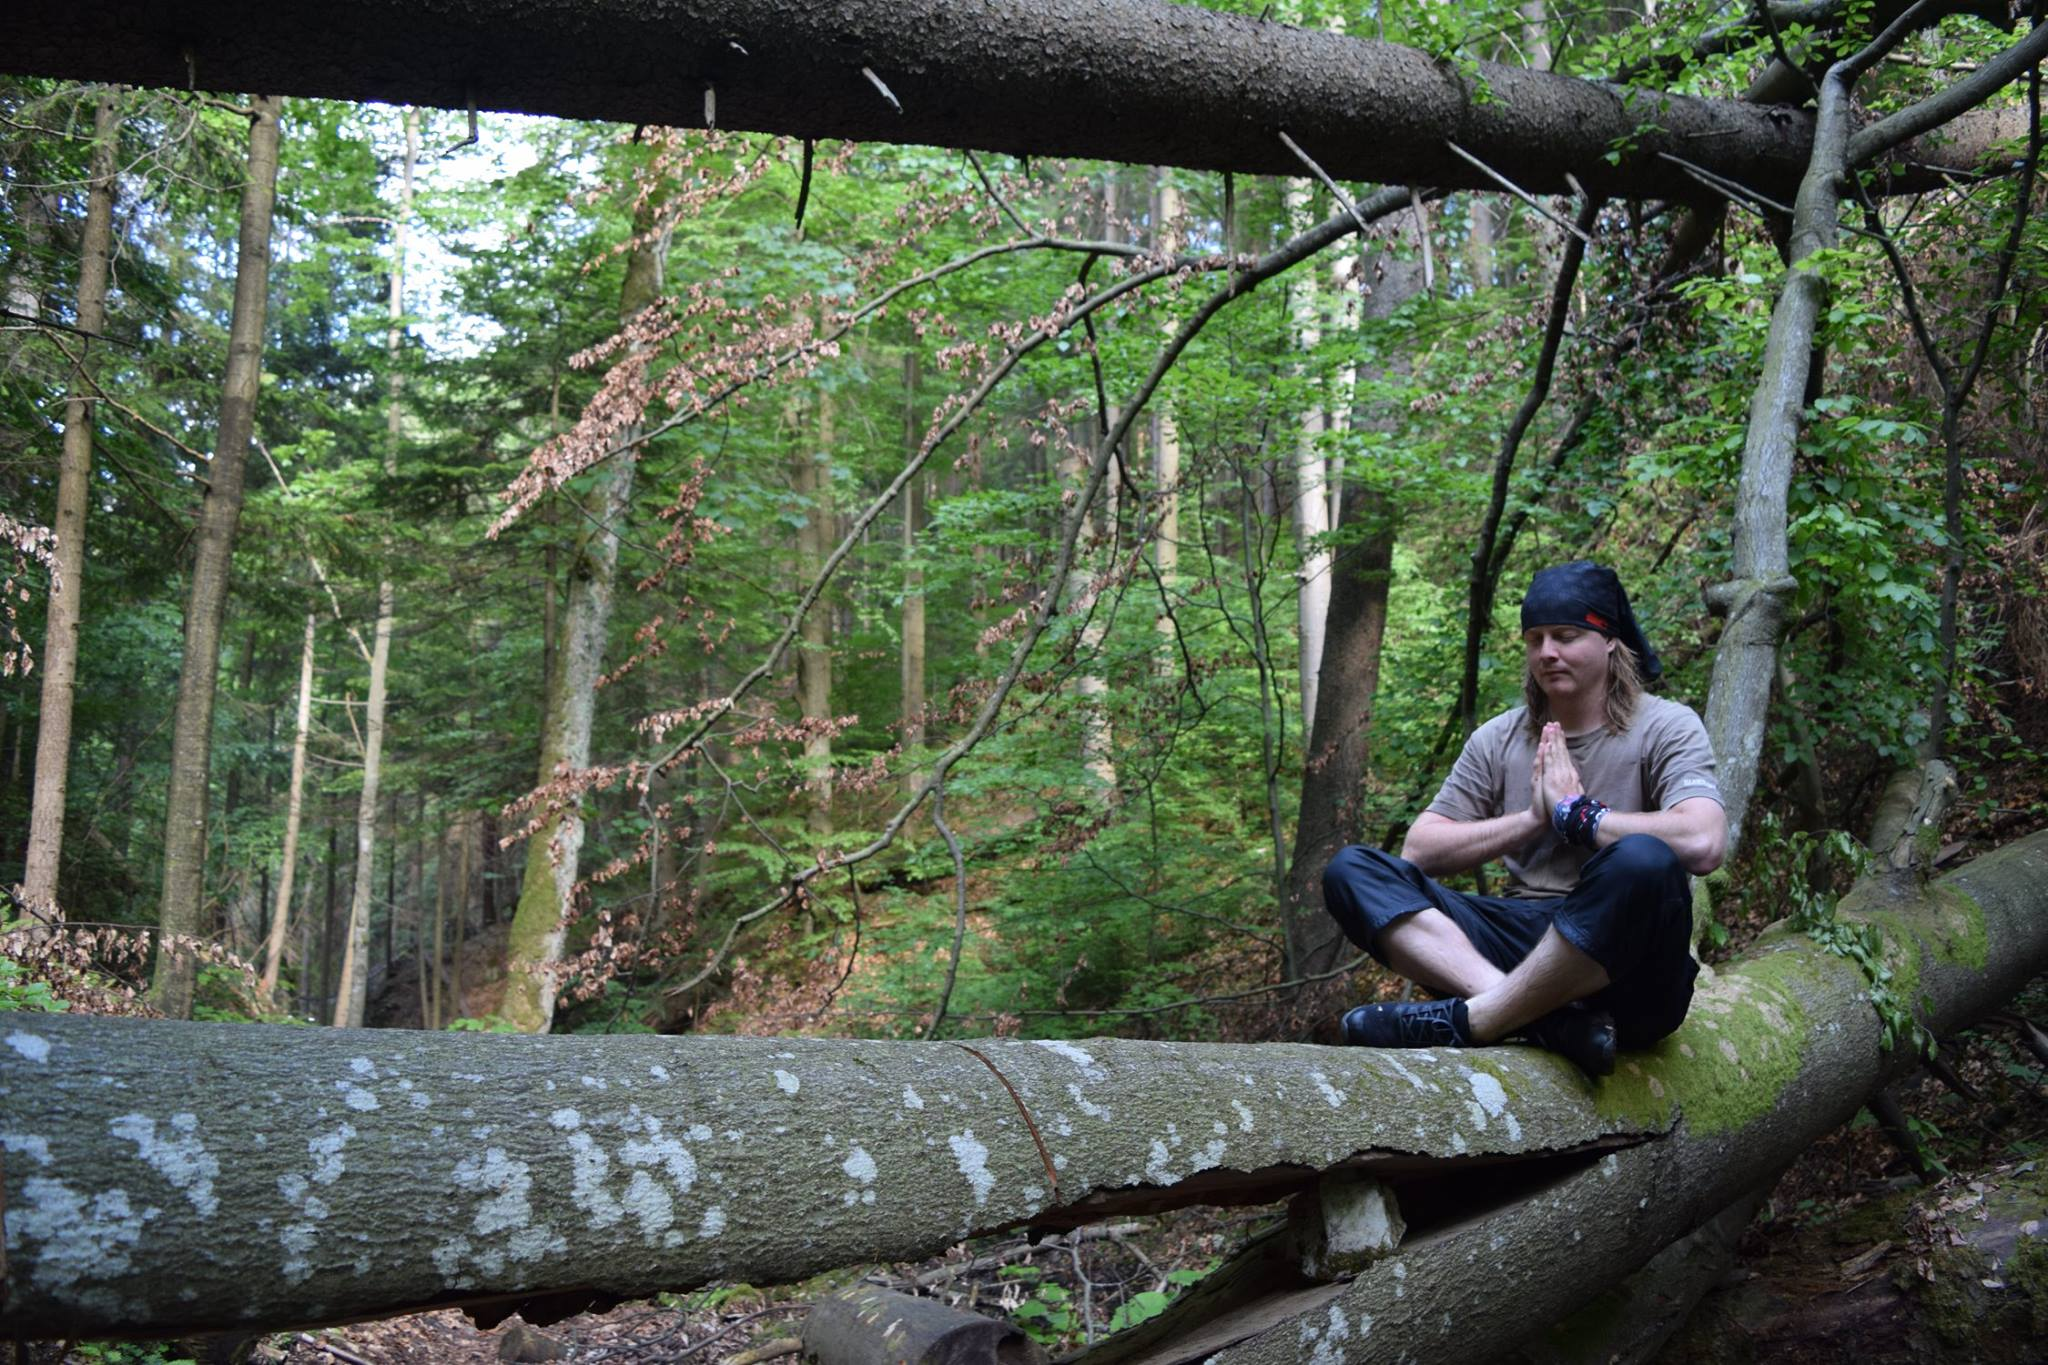
\includegraphics[width=1.0\textwidth]{../../pictures/me.jpg}
\end{center}
\end{minipage}
\end{center}
\end{figure}

\url{https://github.com/michalnand/robotics}
\url{https://github.com/michalnand/machine\_learning}

\centerline{michal.nand@gmail.com}

\end{frame}

\end{document}
